\chapter{Theoretical Review} \label{Cap:theoretical_review}

\begin{displayquote}
    \begin{center}
        \textit{``Do not live bowing down. Die standing up.''}
    \end{center}
\end{displayquote}

\begin{flushright}
   \textit{-- TITE KUBO}
\end{flushright}

\section{Introduction}
This chapter is dedicated to provide a literature review about the Programming Language Design and Compiler/Interpreter Implementation fields. The conceptual content presented here is heavily influenced by \cite{aho1986compilers}, \cite{cooper2022engineering} and \cite{nystrom2021crafting}.

\section{What is a Compiler and How does it work?}
To simply put it simple, a compiler is a software whose responsibility is to translate a program written in a certain programming language into a another program written in another one, without modifying the meaning of the original program, that is, its semantics. However, despite this simple description, compilers are usually complex and large software systems composed of several components which interact with each other during the mentioned translation process, commonly known as compiling.

The importance of compilers in both computer science and real-world applications is immeasurable. The key points below illustrate some of the most prominent impacts of this creation:

\begin{itemize}
    \item \textbf{Bridging High-Level Languages to Machine Code:} As previously mentioned, the purpose of a compiler is the translation between programs written in different programming languages. Usually, in practice, such translation happens from a high-level programming language, commonly more human-readable and that provides several abstractions, into a programming language that is closer to the hardware and, therefore, more machine-readable. Given this fact, it is safe to say that a compiler provides several layers of abstractions that allow developers to build complex software that impact people's life around the world since its conception.
    
    \item \textbf{Impact on Portability:} One of the major features of compilers is their portability. In practice, this means that code once a program, written in a high-level programming language, passes through the compiling process, the resulting machine-code can be used in different hardware platforms by simply targeting different machine architectures, such as: x86, ARM, RISC-V, MIPS and others. This allows the same code base to be re-used in independent systems without the need to rewrite the code base in order to target each different architecture.
    
    \item \textbf{Programming Languages Evolution:} In the current context, it is crucial to reiterate that compilers and programming languages are deeply tied. In practice, the evolution of one serves as a trigger to the evolution of the other and vice-versa. Compilers permit language designers to experiment on new ideas that cross different programming paradigms, such as the procedural, object-oriented, functional, aspect-oriented, concurrent and several others. Furthermore, the evolution of existing programming languages and creation of new ones may allow the enhancement of existing compilers and creation of new ones for niche areas.
    
    \item \textbf{Impact on Software Development:} Without the existence of compilers, the development of software applications would become far more difficult since there would be no bridge uniting codebases written in high-level languages and hardware systems where such codebases are executed. Therefore, this would limit the growth of technology-based companies.
\end{itemize}

Given the impacts emerged from the creation of compilers, now it is time to take a deep dive into how this particular type of software works.

As already explained, a compiler is a complex software system and due to this, must be structurally organized in components responsible for executing a single task in the compiling procedure. According to \cite{cooper2022engineering}, compilers are being implemented since 1955. During these early years of development, a compiler was viewed as a tool that had to understand the program written in the source language and translate it, without altering its meaning, to a target architecture. The distinction between these two tasks, made computer scientist adopt the following structuring when it came down to the components of a compiler: each compiler should have a front-end and a back-end. 

In conformity with what has been exposed, the front-end was responsible for understanding the program written in the source language, while the back-end's responsibility lied on the process of mapping programs to machines. As the reader might have already thought, there must be some kind of link between the front-end and the back-end. That is where the Intermediate Representation (IR) comes in. The front-end must encode the needed information about the source program in some way, so it can be properly used by the back-end when it starts the mentioned mapping process later on. The Intermediate Representation is the entity that contains such information generated by the front-end. It is considered the definitive representation of the source code that will be transformed into machine-code by the back-end.

In short, it can be said that the front-end's responsibility is guarantee that the source code is well-formed and also translate it to the intermediate representation. On the other side, the back-end's duty is translate such intermediate representation into the machine-code of a specific machine architecture, respecting the physical limitations of the target hardware.

As the decades passed on, the process of designing and implementing a compiler became more sophisticated as the structure of such system became increasingly more complex and robust.

Shifting the focus of compilers' implementation to a classroom environment, it is safe to expect that students are capable of implementing more sophisticated compilers that have the following structure, which is not that far from those used in the industry:

\begin{figure}[H]  
  \centering
  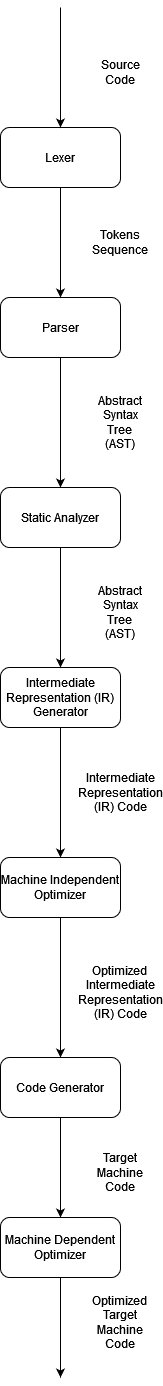
\includegraphics[width=\textwidth, height=0.8\textheight, keepaspectratio]{Figures/Arquiteturas/CompilersDetailedPipeline.png}  
  \caption{A detailed compiler structure}
  \label{fig:comp}
\end{figure}


It is also completely plausible to simplify this task by asking the students to implement a compiler that follows the following simplified structure:

\begin{figure}[H]  
  \centering
  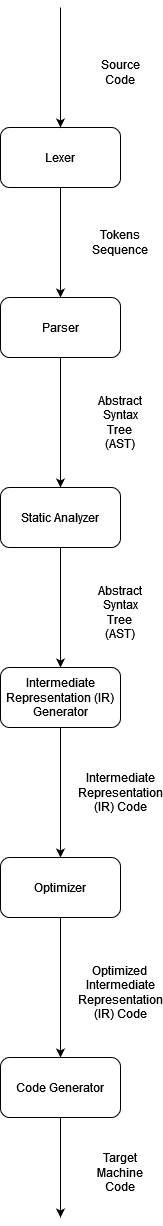
\includegraphics[width=\textwidth, height=0.8\textheight, keepaspectratio]{Figures/Arquiteturas/CompilersSimpliefiedPipeline.png}  
  \caption{A simplified compiler structure}
  \label{fig:Fluxograma}
\end{figure}
    
The next section is dedicated to provide an in-depth overview of each of the compiler's components from the simplified structure presented in the image above.


\section{Detailed Overview of Compiler's Components}

\subsection{Lexer}
The lexer is the first component present in the compiling process of a compiler. It is responsible for executing a process called lexing, which is also known as lexical analysis.

As earlier elucidated, the input of a compiler is the source code of a program written in a specific programming language. The content present inside the source code is viewed by the compiler as a large string, a linear sequence of characters, that has no meaning for it at all at this stage. The lexer's goal is to transform this sequence of characters that is the source code into a new representation that is more abstract from the compiler's perspective, so it can be passed on to the next component, the parser.

To perform such procedure, the lexer takes in this stream of characters and group them together forming a sequence of entities that convey the idea of a "word". These entities are called tokens.

Making an analogy to linguistics, one can say that the lexer's purpose is to group letters (characters) into words (tokens). Given this analogy, it is essential to inform the reader that, like words, tokens can have different lengths and different meanings. Some examples are listed below to better illustrate a few cases:
\begin{itemize}
    \item Single-Character Tokens: \texttt{(}, \texttt{\{}, \texttt{+}, \texttt{-}, \texttt{*}, \texttt{/}, etc.
    \item Double-Character Tokens: \texttt{==}, \texttt{!=}, \texttt{>=}, \texttt{<=}, etc.
    \item Multi-Character Tokens: \texttt{123} (a number literal), \texttt{"hello"} (a string literal), \texttt{true} (a boolean literal), \texttt{aVariable} (an identifier), etc.
\end{itemize}

It is also important to mention that certain characters have no meaning for the lexer during the lexical analysis and, therefore, are completely ignore in the process, such as: whitespace characters and characters that represent comments in the programming language in which the source file was written.

By the end of the lexical analysis, the sequence of characters is transformed into a sequence of tokens by following the syntax rules of the source programming language.

The figure below shows, in an simple example, the input and the output of this component:

\newpage

\begin{table}[h!]
    \centering
    \begin{tabular}{|c|c|c|c|c|c|c|c|c|c|c|c|c|c|c|c|c|c|c|c|c|}
        \hline
        l & e & t &  & a & v & g &  & = & ( & m & i & n & + & m & a & x & ) & / & 2 & ; \\
        \hline
    \end{tabular}
\end{table}

\begin{figure}[h!]
  \centering
  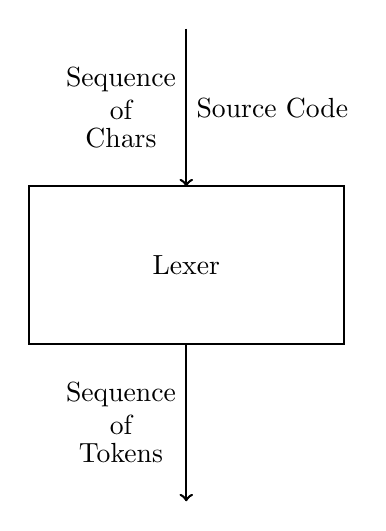
\begin{tikzpicture}
    % Draw the boxes
    \draw[thick] (0, 0) rectangle (4, 2);
    
    % Labels inside the boxes
    \node at (2, 1) {Lexer};

    % Input and output arrows
    \draw[->, thick] (2, 4) -- (2, 2) node[midway, left] {\shortstack{Sequence\\ of\\ Chars}};
    \draw[->, thick] (2, 4) -- (2, 2) node[midway, right] {\shortstack{Source Code}};
    \draw[->, thick] (2, 0) -- (2, -2) node[midway, left] {\shortstack{Sequence\\ of\\ Tokens}};
    \draw[->, thick] (2, 0) -- (2, -2) node[midway, left] {\shortstack{ }};
  \end{tikzpicture}
\end{figure}

\begin{table}[h!]
    \centering
    \begin{tabular}{|c|c|c|c|c|c|c|c|c|c|c|}
        \hline
        let & avg & = & ( & min & + & max & ) & / & 2 & ; \\
        \hline
    \end{tabular}
\end{table}

\begin{figure}[H]  
  \caption{Input and Output of a Lexer}
  \label{fig:lexer}
\end{figure}

As seen in the example above, the lexer receives a sequence of characters, which represents the raw source code, and gives as the result a series of chunks of characters called tokens. Making another analogy with linguistics, one can think of tokens as the "words" and  the "punctuation" that constitutes a programming language.

Going further, it is also possible to say that the lexer's job is execute a traversal through the sequence of characters received and group such characters into the smallest sequences that represent something in the source programming language. Each of these resulting sequences of grouped characters is called a lexeme.

Therefore, in the example presented above, the sequence of lexemes produced from analyzing the sequence of characters received as input was: \texttt{let}, \texttt{avg}, \texttt{=}, \texttt{(}, \texttt{min}, \texttt{+}, \texttt{max}, \texttt{)}, \texttt{/}, \texttt{2}, \texttt{;}

In conclusion, lexemes are just raw substrings presented in the source code.

However, a token is much more than a lexeme. It generally contains other pieces of information that are useful in further stages of the compiling process and also in error report.

Usually, each token has a token type associated. For example, the lexeme \texttt{2} usually has \texttt{NUMBER} as its token type, while \texttt{+} often has \texttt{PLUS} as its token type. In this context, it is relevant to highlight that the amount of token types in a programming language basically depends on the amount of keywords (reserved words) that the language has, the amount of operators at the user's disposal, possibilities of literal values of different data types and, finally, the quantity of delimiters and separators.

Certain types of lexemes have literal values associated with them. numbers, booleans and strings, for example, fall into this category. In these cases, the lexer is able to convert the textual representation of the value into the living runtime entity that might be used by the compiler on later stages of the compiling process.

Last but not least, a compiler must also report errors when it encounters a lexical error during the lexing process, such as: an invalid number literal, an unterminated string, an invalid character that does not follow certain rules of the programming language. In order to report these errors, it is desired that the compiler display as much information as possible to the user about what went and, most importantly, where things went wrong. Having this in mind it is essential to store information about the location of each lexeme in the source code (the line it has appeared and, if possible, its column also).

Now it is time to analyze the functioning of a lexer from an implementation perspective.

The main part of a lexer's code is a loop and variables that are used as "pointers" to keep track of the beginning and ending of each lexeme present in the raw source code file. The lexer then starts working at the first character from the source code and, by using the mentioned "pointers" along with the lexical rules of the source programming language. For the reader that may not be familiar with it, the term "lexical rules" denotes a set of rules that define how characters are grouped to form lexemes in a programming language .Then, it discovers to which lexeme the current character belongs to and consumes any other following characters that also are part of the lexeme. When the end of such lexeme is found, information about its location and literal value are generated and grouped along with the lexeme in order to build and yield the token itself.

This process starts again, in the next iteration of the loop, at the first character that has not been consumed in the generation of the previous token and continues to traverse the source code and generate the corresponding tokens. The lexer continues to do this until it reaches the end of the file. When this happens, it sends the sequence of produced tokens to the next component of the compiler, the parser.

And that is it for lexers. As explained above its implementation is fairly simple and can be done by the programmer without much trouble. In spite of that, it is possible to delegate this task to certain tools, such as: Lex \cite{lesk1975lex} and Flex \cite{Flex}. For the sake of exposition and learning, they work in the following way:

\begin{enumerate}
    \item \textbf{Rule Writing:} When using such tools, the first step is to write the acceptable patters of characters of the source programming language through the use of regular expressions. These regular expressions define the lexemes that are useful and will be used to generate tokens. One example of rule could be "A sequence of digits must be treated as an integer number."
    
    \item \textbf{Lexer Generation and Execution in the C programming language:} Once the rules mentioned in the previous step have been written, the user can run Lex/Flex and the output will be a C program, the lexer that scans the input source code, identifies lexemes and generates the corresponding tokens based on the rules provided.
    
\end{enumerate}

\subsection{Parser}
The Parsing phase of a compiling/interpreting process, also known as Syntax Analysis,

\subsection{Static Analyzer}
The Static Analyzer is the third component present in the compiling process of a compiler. It is responsible for performing a task called static analysis. Static analysis essentially means examining the source code without executing it, hence the name. Delving into it, the static analyzer's task is certify that the source code stick to correctness rules defined by the source programming language design and principles.

Such correctness rules include and are not limited to:
\begin{itemize}
    \item \textbf{Scope and Name Resolution:} This set of rules is responsible for ensuring that variables, functions and classes/types are declared before they are used. In addition, it is also in charge of making the correct bindings between an identifier use and its corresponding declaration, considering the scopes presented in the program's source code.
    
    \item \textbf{Type Checking:} Is an action performed by the static analyzer responsible for ensuring that functions, expressions and variables are properly used. For example: a value of type \texttt{int} cannot be multiplied by a value of type \texttt{bool}, if in a certain function with one parameters expects a value of type \texttt{string}, a value of type \texttt{int} cannot be passed as an argument in a call to such function.
    
    \item \textbf{Detection of Syntax Errors:} Although the parser is responsible for detecting such class of errors, some of these are easier detected during the static analysis stage. For example, a static analyzer can easily detect the misuse of the \texttt{return} keyword outside of a function (default or anonymous) or method. It can also detect the misuse of the \texttt{break} and \texttt{continue} keywords outside of loop statements. There are more examples related to these types of scenarios, but the two mentioned above are good and common examples.
    
    \item \textbf{Detection of Undeclared Variables and Functions:} As the rule's name suggests, a static analyzer is capable of recognizing the usage of variables and functions that have not been previously declared by the developer. It is also worth mentioning, that certain static analyzers take a step beyond and warn the user about variables and functions that have been declared but were never used in the program's source code.
\end{itemize}

Moreover, it is very important to remember the reader that the enforcement of such rules are performed on the Abstract Syntax Tree (AST) provided by the parser in the previous compiling stage, and the output of the static analyzer component is the same, the Abstract Syntax Tree (AST).

Finally, yet importantly, it is important to highlight the fact that in mature compilers (Clang, GCC, javac, Roslyn, rustc, etc.) there is usually more than one static analyzer component. Each of them is responsible for receiving different representations of the program's source code and, consequently, enforce different types of rules according to the philosophy of the source language.

\subsection{Intermediate Representation (IR) Generator}
After the previous phases have been executed

\subsection{Optimizer}
The Optimization phase of a compiling process

\subsection{Code Generator}
The Code Generation phase of a compiling process


\subsection{Virtual Machines}
Virtual Machines are 

\subsection{Runtimes}
Runtimes are


\section{Interpreters}
\subsection{What is an Interpreter?}

\subsection{Compilers and Interpreters}



\section{Shortcuts and Alternate Routes}
This section is dedicated to present an overview of a few alternate ways of implementing a programming language besides the structured route exposed in the previous section. 

This is by no means an exhaustive list of possible approaches to be taken. Instead, it provides an overview of the most common and simple ones.

\subsection{Single-Pass Compilers}
A Single-Pass Compiler

\subsection{Tree-Walk Interpreters}
A Tree-Walk Interpreter

\subsection{Transpilers}
A Transpiler

